




\chapter{Implementation} \label{chap:Implementation}
\section*{Introdution}
%% incomplete
%In this chapter, we will put into practice our proposed approach which is a deep learning model of an IDS that utilises the LSTM algorithm of deep learninglearning

%in the previous chapter in order to test its feasibility and evaluate the results in a study of cases. The objective is to measure the degree of success of our approach. To do this, We will start by proposing a specific 
%XXXXXXX (our specifics)
%which will improve the detection accuracy in smart grid networks

In this chapter, we present our contributions towards the deep learning-based intrusion detection system for the smart grid. due to the fact that smart grid communication requires connecting to the internet, smart grid components now have a new weakness which is cyber-threat. In order to counter this issue, we suggest a deep learning method that utilizes Convolutional Neural Networks (CNNs) and Long Short-Term Memory (LSTM) which is a specific type of Recurrent Neural Network (RNN) to enhance the precision and efficiency of identifying intrusions within the smart grid communication infrastructure.
% mention DoS and DDoS here





\section{Theoretical Proposal}

\subsection{Project Description}
The proposed system for the project is a network intrusion detection system based on deep learning that will depend on either CNN or LSTM models. This project mainly aims at designing and implementing a system that can detect cyber threats in smart grid communication infrastructure effectively. To capture both spatial and temporal features of network traffic data, the proposed system will use either CNN or LSTM architectures to identify complex and sophisticated attack patterns that would threaten the smart grid functionality.
Our deep learning-based network intrusion detection system will be mainly focused on denial of service attacks (DoS) and distributed denial of service attacks (DDoS).

\subsection{Project Design and architecture}
Building any machine learning or deep learning model usually involves several important steps, as shown in Figure  \ref{fig:DL-creation}.


First, we need to collect data that is relevant to the function of the model we want to train, which we will then need to preprocess, which entails clearning, encoding, augmenting, and standardising the data to prepare it for the training phase.


The next step is to select a learning algorithm, the proper optimizer, a loss function, and the evaluation metrics that we will use to train our model.


The model is then trained on the cleaned data, and this is where we feed the trained model new data it has not yet seen before and get the results and predictions on the new data.


The next and final step is the validation step, in which we get the prediction results and evaluate the model accuracy, recall, and f1-score.

\begin{figure}[h]
	\centering
	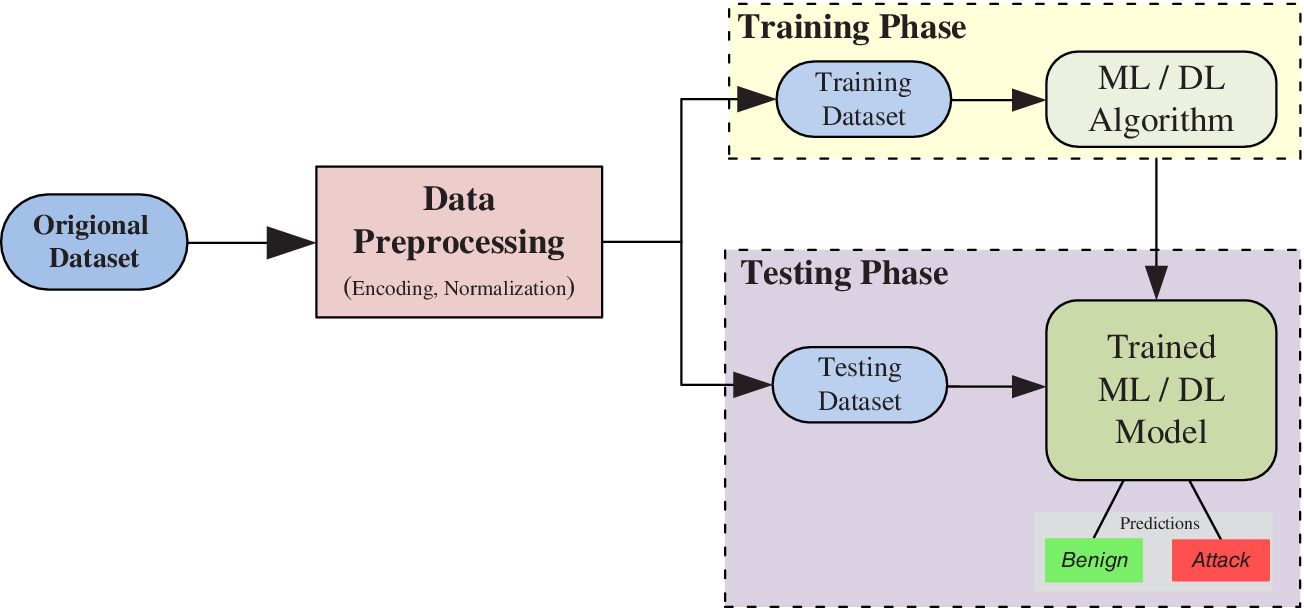
\includegraphics[width=400px]{figures/DL_creation.jpg}
	\caption{deep learning model creation}
	\label{fig:DL-creation}
\end{figure}









\subsection{Deep learning Models architecture}
Detecting cyber threats to the smart grid's functionality and safety is a crucial task that requires high detection accuracy. That's why we opted to use two deep learning algorithms for intrusion detection, which are CNN and LSTM.







%########################			########################################
%########################			########################################
%########################			########################################
%########################			########################################
%########################			########################################



\subsubsection{CNN model}
Convolutional Neural Networks (CNNs) are a highly-specific deep learning algorithm meant to analyze spatialy structured input data, like images and grid structured data. These are derived from the visual cortex of human beings and are good at image recognition, object detection and image segmentation among others. CNNs work by carrying out convolutional layers in order to capture local characteristics, pooling layers in order to reduce spatial dimensions and fully connected layers for predictions. They can be trained on labeled data and have proved very effective in several applications like face recognition, medical imaging analysis as well as self-driving cars.\cite{CNN}
\begin{figure}[h]
	\centering
	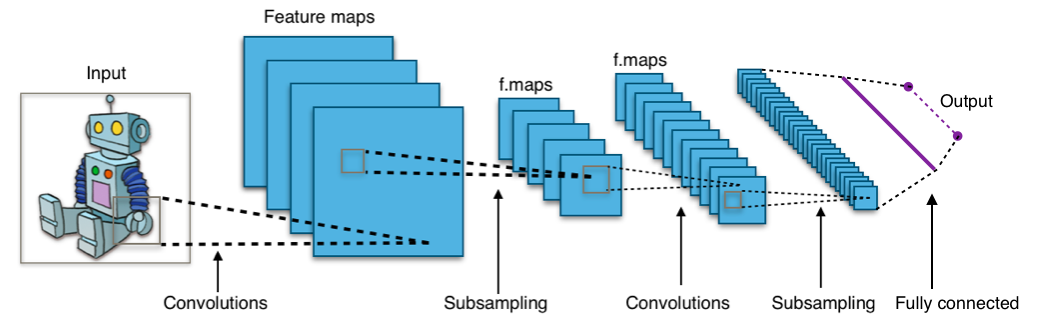
\includegraphics[width=400px]{figures/Typical_cnn.png}
	\caption{CNN architecture \cite{CNN-architecture}}
	\label{fig:CNN-test}
\end{figure}


% add graph
%talk about layers maybe





%########################			########################################
%########################			########################################
%########################			########################################
%########################			########################################
%########################			########################################
%########################			########################################





\subsubsection{LSTM model}
Long Short-Term Memory (LSTM) is a type of Recurrent Neural Network (RNN) that was developed by Hochreiter and Schmidhuber; LSTM is different from RNNs because it can forecast sequences and study long-term dependency patterns from the provided data. What makes LSTMs unique is their ability to learn order dependency patterns which is critical in solving complex problems like speech recognition and machine translation.
LSTM address the weakness of traditional RNN which is the unability to learn any long term patterns which it solves by introducing a memory cell, LSTM is controlled with Three gates control: input gate, forget gate, output gate.These gates determine what information to add, remove, and output from the memory cell and hence enable LSTM networks to learn long-term dependency patterns. \cite{lstm}


\begin{figure}[h]
	\centering
	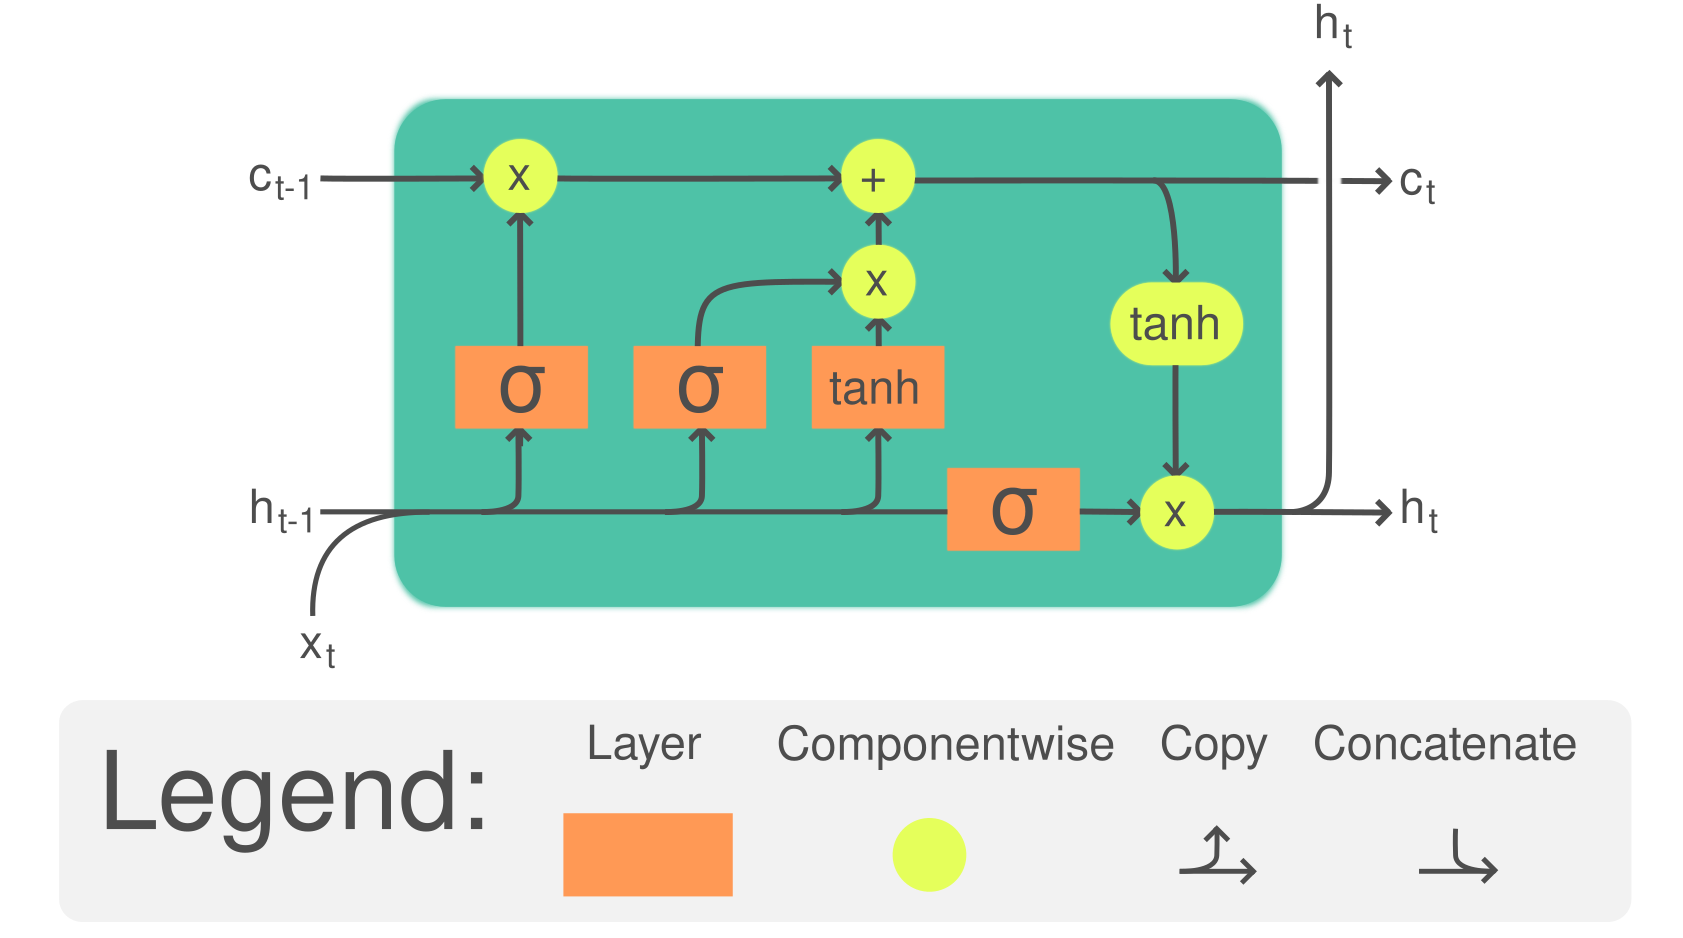
\includegraphics[width=300px]{figures/LSTM_Cell_edited.png}
	\caption{LSTM architecture \cite{LSTM-architecture}}
	\label{fig:LSTM-test}
\end{figure}

% add graph
%talk about layers maybe


%\subsubsection{CNN and LSTM comparison}
%both Convolutional Neural Networks (CNNs) and Long Short-Term Memory (LSTM) have unique advantages and disadvantes, and each of them is well suited to a certain use case, that's why we will be comparing those two models to better understand which one is better suited for a network intrusion detection system.







\newpage
































































































\section{Implementation and Experiments}





\subsection{Development tools used}
\subsubsection{Development environment}
training deep learning models requires a high performance PC due to the fact that these models require high computational resources to process large datasets and intricate neural networks.  With complex calculations and huge amounts of data. One of the reasons why having a powerful PC with a powerful GPU is important during the training process is that it can significantly shorten the time needed for the training, as well as reduce computational resources. a sufficient quantity of memory (RAM) is also needed to load big datasets, and fast storage devices like SSDs are vital in handling data-intensive nature of deep learning tasks. That's why we will be using google colab which has a good selection of hardware for AI training with a top of the line Tesla T4 GPU with 16 GB of VRAM alongside 12 GB of ram and 78GB of disk space.


We will be using two following software for the model's development
\begin{itemize}
	\item jupyter notebook: is an open source web application or a vscode extension that facilitates the creation and sharing of segmented documents that contains blocks of interactive code, text and data visualations, it is mostly used for data science, machine learning and scientific computing, it supports a wide range of programming languages like python, R, scala and julia, it can also display some text formats like markdown and HTML.
	\item VScode: Visual Studio Code (VS Code) is an open-source source-code editor developed by Microsoft for Windows, Linux, macOS, and web browsers. It is a popular choice among developers due to its extensive features like code highlighting, debugging, code completion, and the ability to extend its original functionality with 3rd-party extensions and extensibility. It also offers Git integration out of the box.
\end{itemize}





\subsubsection{programming languages}
The programming language we mainly used is Python 3, important aspect of Python lies in its being more than just an object-oriented programming language because it supports other programming paradigms, which are procedural and functional programming making it flexible when choosing the desired approach. It has user-friendly syntax making it easy to digest even for beginner, This has led to the rise of Python's ecosystem fostered by active community coupled with simplicity behind coding style making it easily accessible by almost everyone. To further improve its capability and functionality, python boast a wide range of third party packages that can easily be installed through Python package manager called pip. Python was created in 1991 by Guido van Rossum. A major landmark came in 2008 with the development of python3 which introduced several improvements and enhancements to the language thereby cementing its place as a valuable flexible programming tool on earth today. \cite{python}

libraries that are used for the development:

\begin{itemize}
	\item NumPy: NumPy is the primary array programming library for the Python language, with an essential role in research analysis pipelines across diverse fields such as physics, chemistry, astronomy, geoscience, biology, psychology, and more. The NumPy array is an efficient data structure that stores and accesses multidimensional arrays (tensors), enabling a wide variety of scientific computation. NumPy was initially developed by students, faculty and researchers to provide an advanced, open-source array programming library for Python, with a sense of building something consequential together for the benefit of many others. \cite{python}



	\item Pandas: Pandas is a Python open source program meant for data management and analysis, it was started in 2008 by AQR Capital Management. It went public in late 2009 and has an active community of contributors. Some of the most important features associated with pandas are fast and efficient DataFrame object for data manipulation with integrated indexing, tools for reading and writing data between in-memory data structures and different formats, time series functionality like date range generation, frequency conversion, moving window statistics, and date shifting and highly optimized performance with critical code paths written in Cython or C. \cite{pandas}
	

	
	\item Matplotlib: Matplotlib is a 2D plotting library for Python which can produce publication quality plots, used in application development, interactive scripting and image creation on all operating system and user interface platforms. The author of Matplotlib John D. Hunter began using Python in 2001 and was initially frustrated at the lack of a powerful graphics environment like MATLAB's. He then developed Matplotlib to satisfy his needs, focusing initially on embedding it in a GUI for his ECoG application and then gradually adding support for other features like high-quality raster and vector output, support for mathematical expressions, and interactive use from the shell.\cite{plot}


	\item Seaborn: Seaborn is a python library for making statistical graphics, Seaborn is a high-level interface to Matplotlib and compatible with Pandas's data structures. Many Seaborn functions can generate multi-panel figures for comparing different subsets of data or variable pairings within a dataset. By allowing quick prototyping and exploratory analysis of data in single-function calls with just a few arguments, Seaborn can be used throughout the scientific project cycle.  \cite{seaborn}
	%\item Seaborn: Seaborn is a python library for making statistical graphics, Seaborn is a high-level interface to Matplotlib and compatible with Pandas's data structures. Seaborn can provide the data with a dataset alongside plot specifications and automatically maps the values onto visual attributes such as color, size or style; internally seaborn performs the relevant statistical transformations and finally adds axis labels as well as legends for the plots. Many Seaborn functions can generate multi-panel figures for comparing different subsets of data or variable pairings within a dataset. By allowing quick prototyping and exploratory analysis of data in single-function calls with just a few arguments, Seaborn can be used throughout the scientific project cycle.  \cite{seaborn}

	\item scikit-learn: Sckit-learn is a Python library that provides various machine learning algorithms for medium-scale supervised and unsupervised problems. It focuses on making things easy, having good performance, documentation and remaining consistent in it's APIs. Scikit-learn depends on scientific Python ecosystem libraries such as NumPy and SciPy, and uses Cython to blend C/C++ with Python for improved performance. it is distributed under a simplified BSD license.\cite{scikit-learn}
	%\item scikit-learn: Sckit-learn is a Python library that provides various machine learning algorithms for medium-scale supervised and unsupervised problems. It focuses on making things easy, having good performance, documentation and remaining consistent in it's APIs. Scikit-learn depends on scientific Python ecosystem libraries such as NumPy and SciPy, and uses Cython to blend C/C++ with Python for improved performance. This lightweight software has few requirements and can be obtained by anyone without any major legal challenges since it is distributed under a simplified BSD license. It provides solid implementations of Machine Learning algorithms, documentation and community driven development, scikit-learn also includes some nice implementations of different algorithms outperforming other popular python ML libraries in many instances including SVMs, Lasso, Elastic Net, k-Nearest Neighbors, PCA, k-Means and some other algorithms.\cite{scikit-learn}


	\item TensorFlow: TensorFlow is a free and open-source software library for machine learning and artificial intelligence. It gives you more flexibility and control the some of the other machine learning frameworks with features such as the Keras Functional API and the Sub-Classification API model to build complex neural network topologies. it offers fast execution for fast debugging and simple prototyping.\cite{tf}
	

	\item Keras: Keras is an open-source library that provides a Python interface for artificial neural networks. Keras was first independent software, then it was integrated into TensorFlow library, and later started supporting others like AJX and PyTorch.\cite{keras}




	

\end{itemize}






%################################################################
%################################################################
%################################################################
%################################################################
%################################################################
%################################################################
%################################################################
%################################################################
%################################################################
%################################################################
%################################################################
%################################################################
%################################################################
%################################################################
%################################################################











\subsection{Dataset}\label{Dataset}
The IDS 2018 dataset is the data set used for this project, this dataset is a comprehensive and realistic dataset for intrusion detection systems. it was created through a collaboration effort between the Communications Security Establishment (CSE) and the Canadian Institute for Cybersecurity (CIC). It includes a few types of attacks such as Brute-force, Botnet, DoS, DDoS and Web attacks, also network infiltration from within all of which are a common attack on smart grid systems. This resulted in 16,233,002 traffic samples which were collected over 10 days from ten real networks, an unusual feature of this data set is its imbalance in benign to malicious ratio of cases. The CICFlowMeter-V3 generates 80 features extracted from the network traffic which describe various intrusions along with abstract distribution models for applications, protocols or even lower level networking entities. Researchers widely employ this dataset to analyze their IDS performance in different research works while others use it to build advanced IDS models. This dataset is not specific to smart grid activity but it is a generalized dataset that includes generalized network traffic which would be the same in a smart grid.




\subsection{Data preprocessing}
Data preprocessing is a crucial step, and the first step in training a machine learning model is data preprocessing. It involves cleaning, transforming, and organising the dataset before it can be used by the machine learning algorithms. Data preprocessing entails improving dataset quality by addressing issues such as missing values, invalid values, and inconsistencies. Data preprocessing techniques include cleaning the data to get rid of errors, normalising the data so that features have the same scale, and feature engineering, which will result in new informative variables, augmenting the data, and resampling it to avoid bias in our model. Preparing the data effectively ensures that machine learning models can accurately learn patterns, increasing their performance and, hence, more accurate results.



\subsubsection{importing data}
First, we load the data with the Pandas library, and since our dataset is split into 10 files, we load the files that include the data related to DoS and DDoS attacks, and we merge the data into the same variable for easier preprocessing while deleting the old variable to avoid uselessly filling the memory. We also remove an unneeded column from one of the dataset files.

\lstinputlisting[language=Python, caption={loading data}]{listings/loading_data.py}

The total amount of data loaded is about 11 million rows with 80 columns, all of which are either benign or DoS/DDoS traffic, with a total size of 6.6 GB.

\newpage


\begin{figure}[h]
	\centering
	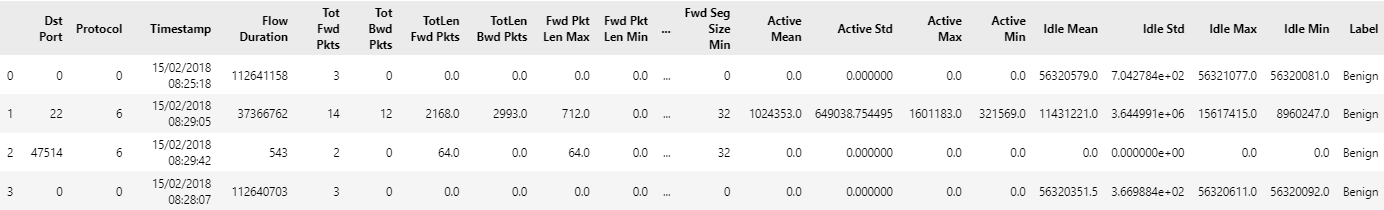
\includegraphics[width=400px]{figures/data_example.png}
	\caption{Imported data sample}
	\label{fig:datasample}
\end{figure}

As we can see in Figure \ref{fig:unbalanced_data} and Table \ref{tab:unbalanced_data_table} below, the data is unbalanced, but we will fix that later in the data preprocessing phase, specifically in the data augmentation phase.

\begin{figure}[h]
	\centering
	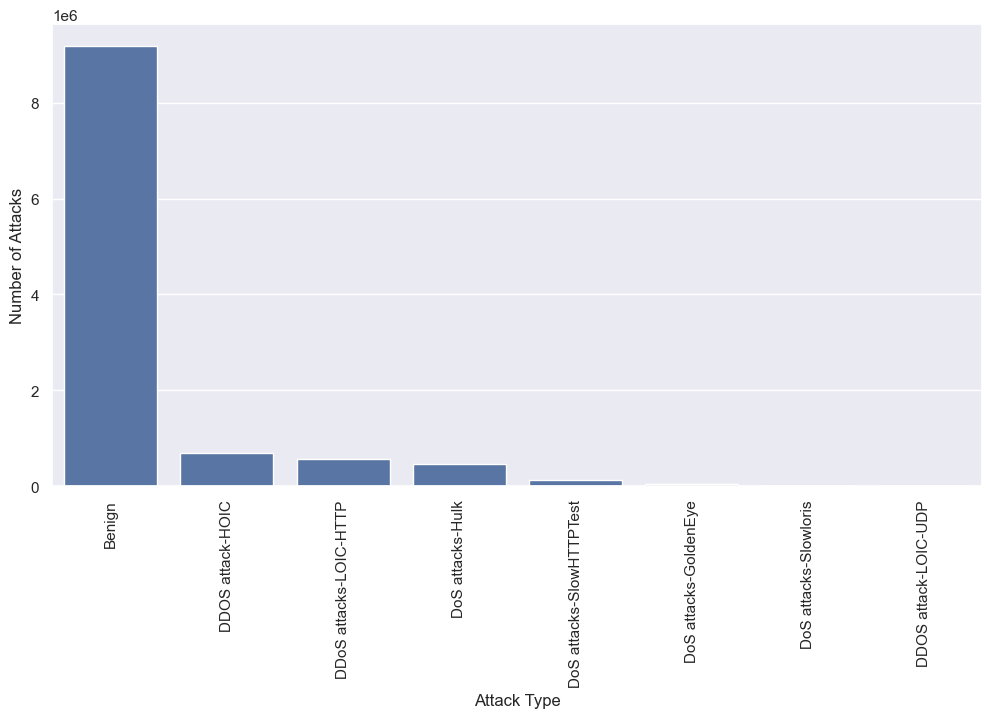
\includegraphics[width=400px]{figures/unbalanced_data.png}
	\caption{Bar graph of the unbalanced dataset}
	\label{fig:unbalanced_data}
\end{figure}

\begin{table}[h]
	\centering
	\caption{the number of occurrence for each traffic type}
	\begin{tabular}{|p{6cm}|p{6cm}|}

\hline activity type & number of ocurences \\
\hline Benign & 9176239 \\
\hline DDOS attack-HOIC & 686012 \\
\hline DDoS attacks-LOIC-HTTP & 576191 \\
\hline DoS attacks-Hulk & 461912 \\
\hline DoS attacks-SlowHTTPTest & 139890 \\
\hline DoS attacks-GoldenEye & 41508 \\
\hline DoS attacks-Slowloris & 10990 \\
\hline DDOS attack-LOIC-UDP & 1730 \\
\hline

\end{tabular}

	\label{tab:unbalanced_data_table} 
\end{table}

\newpage

\subsubsection{Cleaning data}
This is an important step, and executing it efficiently is necessary for accurate predictions in our deep learning model. To clean our data, we must first find and remove unwanted data like missing values, null values, duplicate rows, and unneeded columns or features.



\firmlist
\begin{itemize}
	\item Finding and cleaning missing values: First, we identify the columns that contain null values in our dataset by identifying columns with missing values, after which we decide to eliminate the rows containing null values from the dataset. The objective of this step is to eliminate missing data to ensure quality and consistency in the model training.
	\lstinputlisting[language=Python, caption={Cleaning data}]{listings/cleaning_nulls.py}
	\item Removing duplicate rows: We also remove duplicate rows for a better-quality dataset and to avoid bias in our model.
	\lstinputlisting[language=Python, caption={Removing duplicates}]{listings/cleaning_dups.py}
\end{itemize}






\subsubsection{Encoding the categorical variables}
The LabelEncoder assigns a unique integer to each categorical value, which is the label in our case, which is the traffic type (benign or attack type), which allows them to be represented in a numerical form. This makes it easier to use these variables in machine learning algorithms, as they can handle numerical values better.


\lstinputlisting[language=Python, caption={Encoding the categorical variables}]{listings/encoding_cat_var.py}






\subsubsection{Augmenting the data}
As we have stated before in Section \ref{Dataset}, our dataset is unbalanced in the distribution between benign and malicious activity, which is a bad thing because it will introduce bias, overfitting, and poor prediction performance to our model. Therefore, In this step, we will resample our dataset to get a better 1:1 ratio between our different categorical variables (benign and other attack types). The following Python code snippet uses the resample function from scikit-learn; it does the resampling we need to make our dataset balanced.




\lstinputlisting[language=Python, caption={resampling the dataset}]{listings/resample.py}



\begin{itemize}
	\item \texttt{data\_X}:  All of those variables are our data, which has been cleaned and separated according to the categorical variables that we previously encoded.
	\item \texttt{n\_samples}: Is the number of rows for each attack type; in this case, we used 20000 rows.
	\item \texttt{random\_state}: This is the resampling seed; by using the same seed number, we can ensure that we always get the same results.
	\item replace: This variable decides whether or not a sample can be selected multiple times.
\end{itemize}



% change to pie and change colors
\begin{figure}[h]
	\centering
	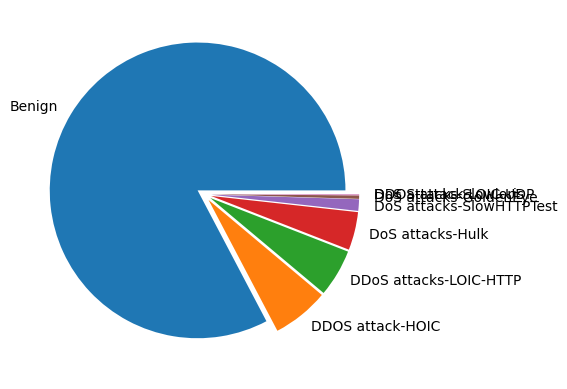
\includegraphics[width=350px]{figures/unbalanced_donut.png}
	\caption{Before data augmentation}
	\label{fig:datasample}
\end{figure}
\begin{figure}[h]
	\centering
	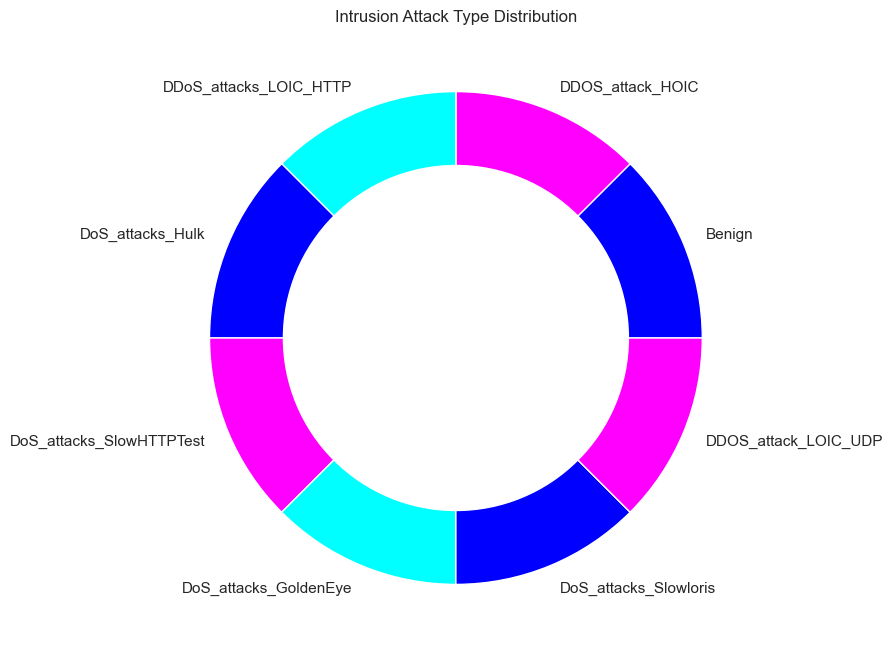
\includegraphics[width=350px]{figures/balanced_donut.png}
	\caption{After data augmentation}
	\label{fig:datasample}
\end{figure}

Those resampled variables are then merged and fed to the deep learning model for training.

% this part's format is broken the pdf file





\subsubsection{splitting the data for the deep learning model}
% this part needs to be extended
In this step we split our data into 2 sets, training and testing sets:
\begin{itemize}
	\item training data: 90\% of the total dataset
	\item testing data 10\% of the total dataset
\end{itemize}
\lstinputlisting[language=Python, caption={Splitting the dataset}]{listings/data_split.py}
















%##############################################################
%##############################################################
%##############################################################
%##############################################################
%##############################################################
%##############################################################
%##############################################################
%##############################################################
%##############################################################
%##############################################################
%##############################################################
%##############################################################
%##############################################################
%##############################################################





\subsection{Deep learning models implementation}




\subsubsection{CNN model}
% something here
In this step we implement a Network Intrusion Detection System (NIDS) using a Convolutional Neural Network (CNN) deep learning model. The model, defined with the Keras Sequential API, is made up of several convolution and pooling layers followed by fully connected layers. The CNN has been structured such a way that it is able to recognize network traffic data patterns meaning it can detect and classify potential denial-of-service (DoS) and distributed denial-of-service (DDoS) attacks.


CNN deep learning model creation using the Kera API functions:
\lstinputlisting[language=Python, caption={CNN Model creation}]{listings/CNN_model.py}

\firmlist
\begin{itemize}
	\item Sequential(): Creates a model with a stack of layers, where each layer has one input and one output.
	\item Conv1D(): Adds one dimensional convolutional layer to the model, results in an output tensor.
	\item MaxPooling1D(): It adds a pooling operation to one-dimensional temporal data.
	\item Flatten(): This function is used to flatten a matrix into a one-dimensional array.
	\item Dense(): Previous layer outputs given as inputs to it's neurons, with each nruron producing only one output for the next layer.
	\item BatchNormalization(): It is employed to normalise the input data such that the mean output is close to zero and the output standard deviation is close to one.
	\item compile(): Is used for configuring the model before training; this includes but is not limited to:
		\firmlist
		\begin{itemize}
			\item loss function: categorical crossentropy, which calculates cross-entropy loss between labels and predictions.
			\item optimizer: Adam optimization. Stochastic gradient descent method based on adaptive estimation of first-order and second-order moments.
			\item metrics: accuracy is the ratio of correct predictions to the total number of predictions.
		\end{itemize}
\end{itemize}


We also get a summary of the created model. This summary describes the arrangement of the model layers, the number of parameters in each layer, the output shape of each layer, and the number of trainable and non-trainable parameters.



\newpage

\begin{figure}[h]
	\centering
	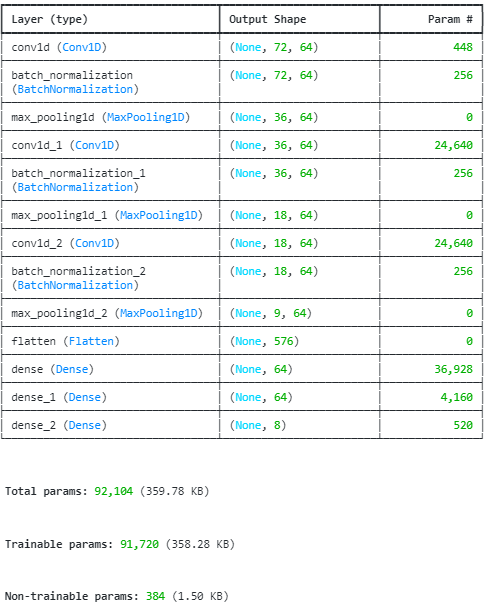
\includegraphics[width=300px]{figures/CNN_model_summary.png}
	\caption{CNN model summary}
	\label{fig:test}
\end{figure}

% add graph
% reùove this title and continue

The next step is starting the model training with 30 epochs, 32 batch sizes, and the validation data, which is the test data we split from the original dataset earlier.


\lstinputlisting[language=Python, caption={Start the CNN model training}]{listings/CNN_training.py}


After the training process is finished, we can use the Keras save() function to save our train model into a .keras file for later use, so we can reuse our model without having to train it each time.


\lstinputlisting[language=Python, caption={Saving the CNN model}]{listings/CNN_save_load_model.py}


%here we add the saving the model






%##############################################################
%##############################################################
%##############################################################
%##############################################################
%##############################################################
%##############################################################
%##############################################################
%##############################################################
%##############################################################
%##############################################################
%##############################################################
%##############################################################
%##############################################################
%##############################################################






\subsubsection{LSTM model}
% say something
The LSTM model implementation is very similar to the CNN implementation, with only a few challenges. Those changes being that CNN uses the Conv1D() function to create its one-dimensional convolutional layer, while LSTM uses the LSTM() function to add its layers.

\lstinputlisting[language=Python, caption={LSTM model code}]{listings/LSTM_model.py}
And after the model training is finished, we save the model for later loading and usage.
\lstinputlisting[language=Python, caption={Saving the LSTM model}]{listings/LSTM_save_load_model.py}
\newpage

We get a model summary for the LSTM model as well.

\begin{figure}[h]
	\centering
	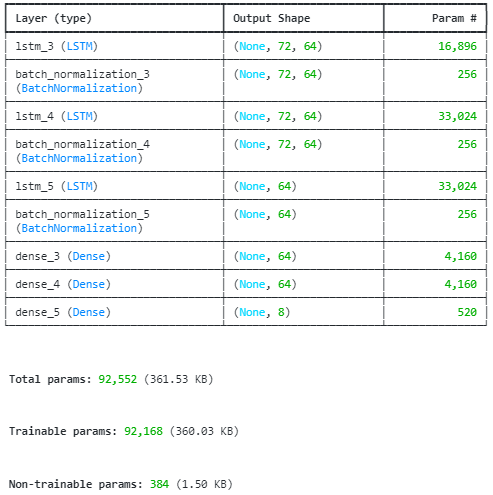
\includegraphics[width=400px]{figures/LSTM_model_summary.png}
	\caption{LSTM model summary}
	\label{fig:test}
\end{figure}


%here we add the saving the model











\subsection{Results}
In this step, we will compile the data from our model evaluation on the test data with both the CNN and the LSTM models. The metrics that we use for evaluation are mainly the detection accuracy and loss rate. We will also be looking at other metrics like

The metrics used for the evaluation are primarily accuracy, but there are also some other metrics, including:
\begin{itemize}
	\item Accuracy: Accuracy is a measure of the overall correctitude of predictions made by models. It can be calculated as (TP+TN)/(TP+TN+FP+FN). The accuracy metric is deceptive especially in cases where datasets are not balanced.
	\item precision: Precision on the other hand measures the rate of true positives among all positive predictions that the model makes. Precision can be expressed as TP/(TP+FP). Precision comes in handy when wrong positive consequences could have serious implications, for example spam detection effort.
	\item F1-score: F1 score is harmonic mean of precision and recall and ranges between 0 to 1 whereby 1 means best. F1 Score provides balance between recall and precision. This may be given as 2*(Precision*Recall)/(Precision + Recall).
	%\item confucsion matrix: A confusion matrix is a table that summarizes how well a classifier performed in classification tasks. In one axis there are actual values while on another predicted values are found. These cells consists of True Positives(TP), True Negatives(TN), False Positives(FP) and False negatives (FN).
\end{itemize}












\subsubsection{CNN model}
evaluating the CNN model with the test data:
\firmlist
		\begin{itemize}
			\item accuracy:
				\begin{itemize}
					\item Training accuracy: 99.6\%
					\item Validation accuracy: 98.17\%
				\end{itemize}
			\item loss:
				\begin{itemize}
					\item Training loss: 1.54\%
					\item Validation loss: 7.05\%
				\end{itemize}
		\end{itemize}


		
		\lstinputlisting[language={}, caption={CNN multilabel classification report}]{listings/CNN_report.txt}



		\newpage
		% add recall precsition and f1-score
		% add confucsion matrix
		% images

		% show 3 last epochs 
		% show 2 graphs


		\begin{figure}[t]
			\centering
			\begin{minipage}{0.4\textwidth}
			  \centering
			  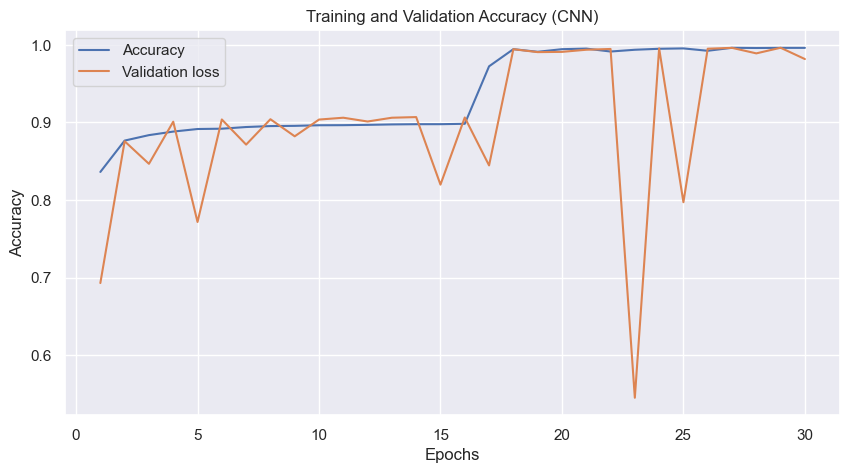
\includegraphics[width=1\textwidth]{figures/CNN_training_validation.png}
			  \caption{CNN Accuracy graph}
			  \label{fig:1}
			\end{minipage}
			\hfill
			\begin{minipage}{0.4\textwidth}
			  \centering
			  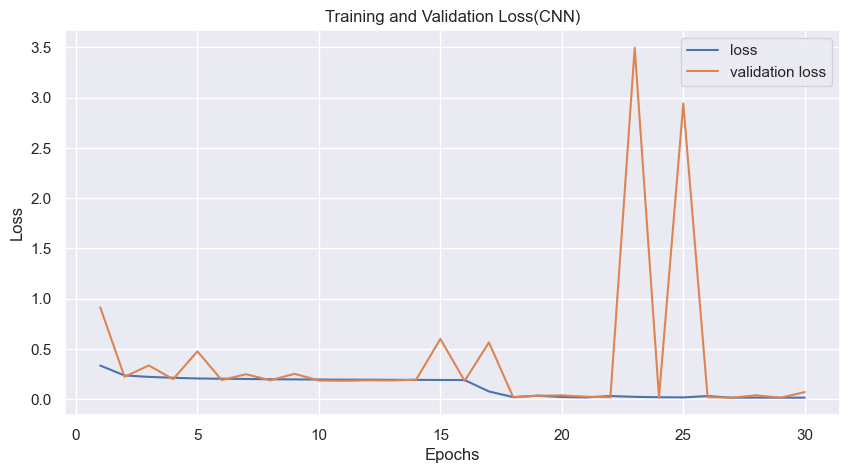
\includegraphics[width=1\textwidth]{figures/CNN_training_validation_loss.png}
			  \caption{CNN Loss graph}
			  \label{fig:2}
			\end{minipage}
		\end{figure}


		%\begin{figure}[h]
		%	\centering
		%	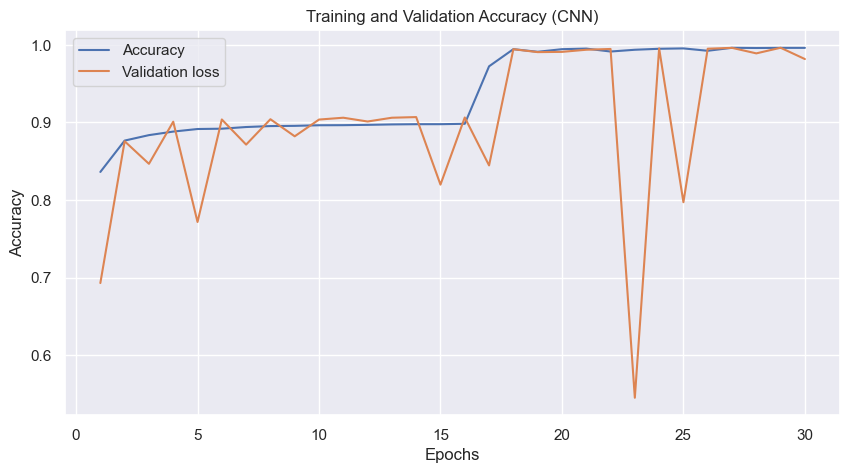
\includegraphics[width=400px]{figures/CNN_training_validation.png}
		%	\caption{Accuracy graph}
		%	\label{fig:aa}
		%\end{figure}
		%\begin{figure}[h]
		%	\centering
		%	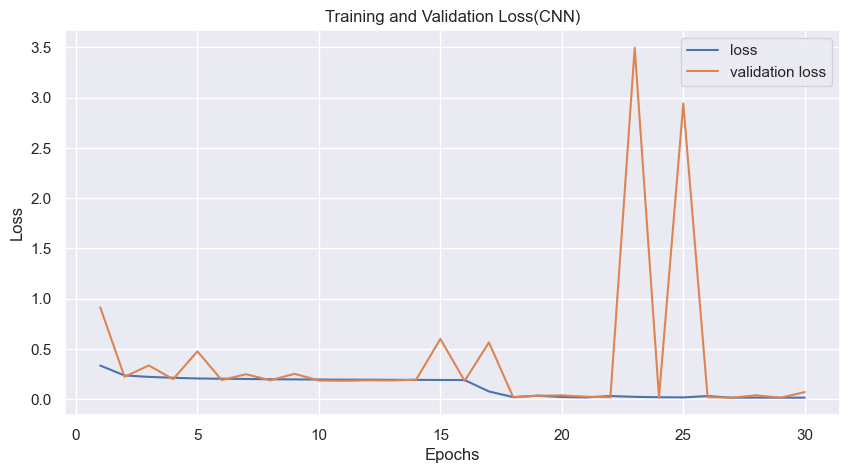
\includegraphics[width=400px]{figures/CNN_training_validation_loss.png}
		%	\caption{Loss graph}
		%	\label{fig:ff}
		%\end{figure}
		


\subsubsection{LSTM model}


evaluating the LSTM model with the test data:
\firmlist
		\begin{itemize}
			\item accuracy:
				\begin{itemize}
					\item Training accuracy: 99.6\%
					\item Validation accuracy: 99.65\%
				\end{itemize}
			\item loss:
				\begin{itemize}
					\item Training loss: 1.72\%
					\item Validation loss: 1.48\%
				\end{itemize}
		\end{itemize}
		\lstinputlisting[language={}, caption={LSTM multilabel classification report}]{listings/LSTM_report.txt}
		
		% add recall precsition and f1-score
		% add confucsion matrix
		% images

		% show 3 last epochs 
		% show 2 graphs


		\begin{figure}[t]
			\centering
			\begin{minipage}{0.49\textwidth}
			  \centering
			  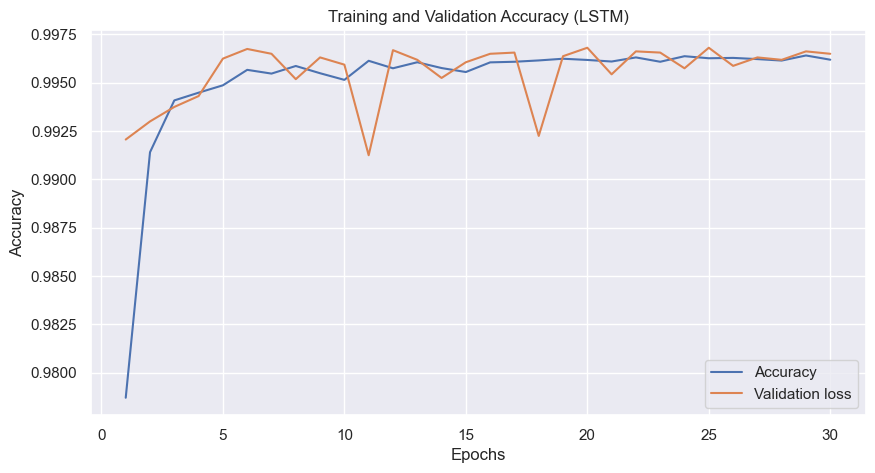
\includegraphics[width=1\textwidth]{figures/LSTM_training_validation.png}
			  \caption{LSTM Accuracy graph}
			  \label{fig:1}
			\end{minipage}
			\hfill
			\begin{minipage}{0.49\textwidth}
			  \centering
			  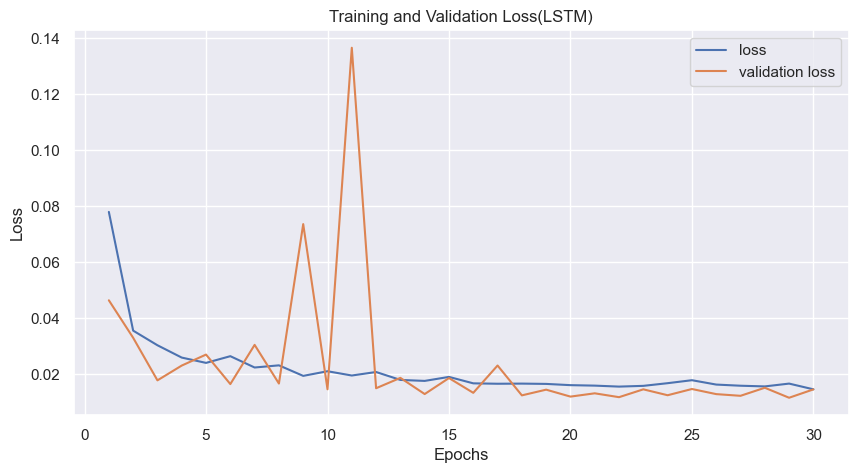
\includegraphics[width=1\textwidth]{figures/LSTM_training_validation_loss.png}
			  \caption{LSTM Loss graph}
			  \label{fig:2}
			\end{minipage}
		  \end{figure}
		  
		  \newpage

%
%		\begin{figure}[h]
%			\centering
%			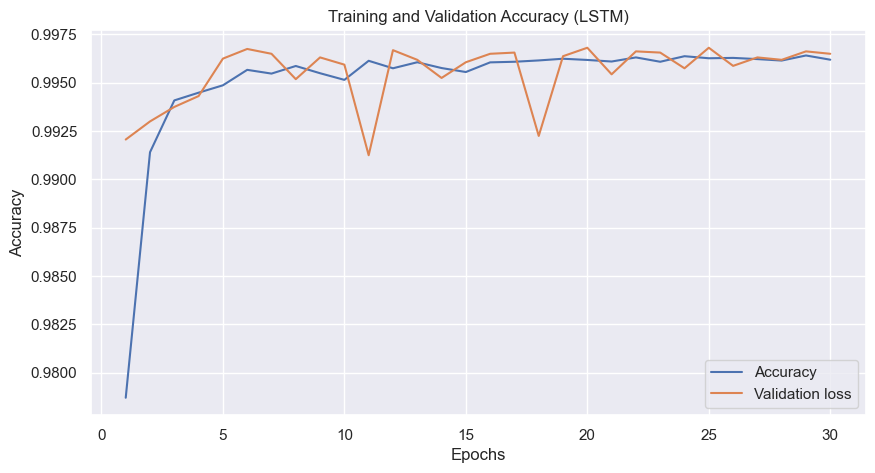
\includegraphics[width=400px]{figures/LSTM_training_validation.png}
%			\caption{Accuracy graph}
%			\label{fig:aa}
%		\end{figure}
%% to avoide funky layout
%\newpage
%		\begin{figure}[h]
%			\centering
%			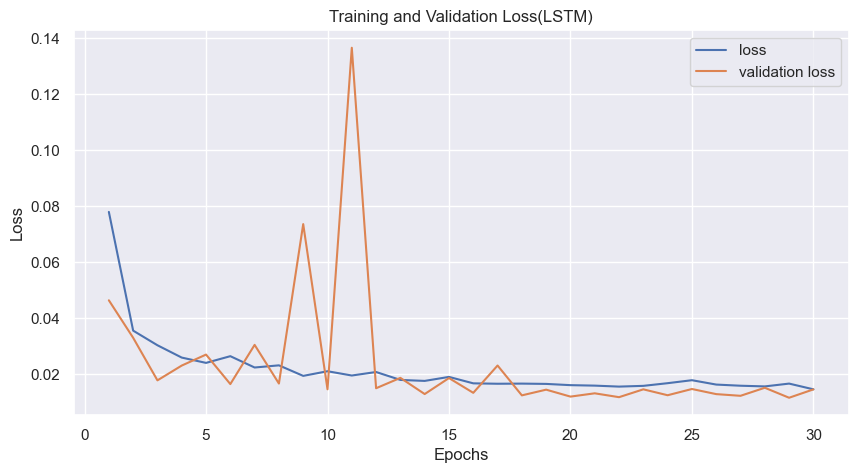
\includegraphics[width=400px]{figures/LSTM_training_validation_loss.png}
%			\caption{Loss graph}
%			\label{fig:ff}
%		\end{figure}
		




% fix me between ()
\paragraph{Observation}: We notice that the accuracy and loss rates between the CNN and the LSTM models were better, but only with a slight difference. We also notice that CNN also takes more epochs to reach its maximum performance. Also,  according to the validation accuracy compared to the number of epochs, the LSTM provides better accuracy over a wider range of epochs, while CNN provides its best accuracy over a narrower range of epochs.

		







\subsection{Conclusion}
In this chapter we demonstrated the development of two different deep learning methodes for creating a network intrusion detection system that protects the smart grid from DoS and DDoS attacks, starting with the development environment, the architecture of the used algorithms, and the data preprocessing, cleaning and training the models, and finishing the chapter with a performance comparison between the two models.





\newpage












